% !TEX root = ../Main.tex

\chapter{Stabilizer Decompositions of Quantum States}\label{chap:stabrank}
\section{Introduction}\label{sec:decomposition_intro}
%Connect back to `resource theory' ideas
%Expand circuit/circuit state in terms of a free resource, here stabilizers
In the previous chapter, we discussed in detail efficient simulations of stabilizer circuits. Recalling the discussion in Section\textbf{Please insert your reference later}, this classical simulability in turn implies that non-stabilizer states are a resource for quantum computation. In this section, we will introduce a particular model of quantum computation that makes explicit the computational role of `magic' states, Pauli Based Computation~\cite{Bravyi2015,Yoganathan2019}.\par
This model forms the basis for the definition of Stabilizer Rank, a quantity which tries to relate the computational power of non-stabilizer states to the task of classical simulation. This chapter will be focused on extending the stabilizer rank method, whereas the following chapter will focus on its implementation for the task of classical simulation.
\subsection{Pauli Based Computations}
A Pauli Based Computation (PBC) is a measurement-based model of quantum computing, whereby a computation is realised by applying a sequence of Pauli measurements to a set of non-stabilizer magic states, and post-processing of the measurement outcomes. In general, this sequence will be `adaptive', and the choice of measurement operator will depend on the outcome of previous measurements.\par
It is well known that quantum circuits built out of Clifford gates and the $T$ gate are universal for quantum computation~\cite{Bravyi2005}. Thus, any arbitrary computation $U$ acting on a computational input state can be expressed as a circuit with $m$ Clifford operations and $t$ $T$ gates.\par
\begin{figure}[t]
\centering
\centerline{
\begin{subfigure}[t]{0.45\textwidth}
\centering
$
\Qcircuit @C=1em @R=.7em {
    \lstick{\ket{0}} & \gate{H} & \ctrl{1} & \gate{T} & \qw & \measureD{Z}\\
    \lstick{\ket{0}} & \qw & \targ & \gate{T} & \gate{S} & \measureD{Z}\\
}
$
\end{subfigure}
\begin{subfigure}[t]{0.55\textwidth}
\centering
$
\Qcircuit @C=.3em @R=.7em {
\lstick{\ket{0}} & \gate{H} & \ctrl{1} & \targ     & \qw       & \meter & \cctrl{2} \\
\lstick{\ket{0}} & \qw      & \targ    & \qw       & \targ     & \meter & \cw       & \cctrl{2} \\
\lstick{\ket{H}} & \qw      & \qw      & \ctrl{-2} & \qw       & \qw    & \gate{C} & \qw       & \qw      & \measureD{Z}\\
\lstick{\ket{H}} & \qw      & \qw      & \qw       & \ctrl{-2} & \qw    & \qw       & \gate{C} & \gate{S} & \measureD{Z}\\
}
$
\end{subfigure}
}
\caption{Figure illustrating two equivalent forms of a small circuit built form the Clifford + $T$ gate set. The lower circuit is obtained from the former by replacing each $T$ gate with a teleportation or `state-injection' gadget that consumes one magic state$\ket{H}=\cos{\frac{\pi}{8}}\ket{0}+\sin{\frac{\pi}{8}}\ket{1}$. This performs a $T$ gate (up to a measurement controlled correction operation $C$ which is a Clifford gate)~\cite{Gottesman1999}.}
\end{figure}
By replacing each $T$ gate in a Clifford+$T$ circuit with a state-injection gadget~\cite{Bravyi2005}, we instead end up with a circuit built exclusively from Clifford gates and Pauli measurements, acting on $n$ qubits in a computational basis state, and $t$ qubits in a non-stabilizer state. Once in this form, we can convert the circuit to a PBC~\cite{Bravyi2015,Yoganathan2019}.\par
In the following discussion, we assume that the only intermediate measurements in the circuit arise from the state-injection gadgets. Circuits with clasically controlled gates condition on intermediate measurements are called `adaptive'. We note that the PBC construction works for both adaptive and non-adaptive circuits, so this assumption can be made without loss of generality~\cite{Bravyi2015,Yoganathan2019}.\par
Once in this form, we can commute every Clifford operator through the circuit and past the final Pauli measurement layer. As we do,  each measurement operator $P\rightarrow P'$ under conjugation, and the Clifford gate can then be discarded as it happens after the measurement layer and thus has no effect on the outcome. These updates can be efficiently computed using the methods discussed in Chapter~\ref{chap:stabilizers}. The result is some new sequence of Pauli measurements $P_{1},\dots,P_{r}$, acting on $n+t$ qubits.\par
It is then possible to show that these measurements can be rearranged such that all measurements commute, and  act non-trivially on only the $t$ magic states. The key technique is a lemma showing that if any pair $P_{j},P_{k}$ anticommute, they can be updated by sampling a measurement outcome $\lambda_{k}=\pm1$ uniformly at random, replacing the $P_{j}$ with a Clifford operator $V_{j,k}=\frac{\lambda_{j}P_{j}+\lambda_{k}P_{k}}{\sqrt{2}}$, where $\lambda_{j}$ was the outcome of measuring $P_{j}$. This Clifford can then be commuted through the rest of the measurement layer~\cite{Yoganathan2019}.\par
Now consider prepending the circuit with Pauli $Z$ measurements on the $n$ computational qubits. By definition, these measurements are deterministic and do not change alter the computation. Application of the above Lemma ensures that these computational measurements all commute with the final measurement operators $P_{i}$, and thus that the $P_{i}$ act trivially on the $n$ computational qubits~\cite{Bravyi2015}.\par
Overall then, the PBC model allows us to realise quantum computation using only a supply of non-stabilizer resource states, Pauli measurements, and probabilistic classical computation, used to compute and update the Pauli measurement sequence~\cite{Yoganathan2019}. The classical component of the computation is efficient, that is to say the measurement sequence can be computed with a runtime that scales polynomially in the number of qubits.\par
A PBC $\mathcal{C}$, obtained from some Clifford + $T$ circuit $U$, can be said to efficiently simulate the original circuit, in both the weak~\cite{Yoganathan2019} and strong sense~\cite{Bravyi2015}. Weak simulation follows immediately as, given a method to sample from the measurement operators of the PBC, this also corresponds to a sample of the output distribution of the original circuit~\cite{Yoganathan2019}. Strong simulation then follows from the result that an adaptive circuit with postselection has a corresponding PBC with postselected Pauli measurements~\cite{Yoganathan2019}. In particular, we can fix both the measurement outcomes of the circuit, and the measurement-controlled correction operations introduced by state-injection. The result is a non-adaptive circuit, which is translated to a non-adaptive PBC with a fixed Pauli projector $\Pi_{x,s}$~\cite{Yoganathan2019}, where $x$ and $s$ are the postselected binary bits corresponding to the measurement outcome and the state-injection gadgets, respectively~\cite{Bravyi2015,Bravyi2016}. The corresponding probability amplitude is thus given by
\begin{equation}
\matrixel{x}{U}{0^{\otimes n}}\equiv 2^{t}\matrixel{T^{\otimes t}}{\Pi_{x,s}}{T^{\otimes t}}
\label{eq:pbc_strongsim}
\end{equation}
where we reweight the probability to account for the fact that each of the $2^{t}$ different outcomes on the state-injection gadgets is equiprobable.
\subsection{Stabilizer State Decompositions}
In the PBC model of quantum computation, the role of non-stabilizer states as a resource for quantum computation is made explicit. It is also clear that the PBC would require exponential time to simulate clasically, as Pauli expectation values on non-stabilizer states cannot in general be efficiently computed~\cite{Gottesman1998b}.\par
In the context of resource theories for quantum computation, we can consider studying quantum computations by decomposing computations in terms of the `free' set of operations. This is what Bravyi, Smith \& Smolin did when considering stabilizer state decompositions of magic states. We define a stabilizer state decomposition of a general state $\ket{\psi}$ as
\begin{equation}
\ket{\psi} = \sum_{i=1}^{\chi}c_{i}\ket{\phi_{i}},
\label{eq:stab_state_decomposition}
\end{equation}
where each $\ket{\phi_{i}}$ is a stabilizer state and the total number of terms in the decomposition, $\chi$, is called the \emph{Stabilizer Rank} of the state $\ket{\psi}$.\par
Given a PBC, and a stabilizer state decomposition of the magic states $\ket{T}^{\otimes t}$, then strong simulation of a PBC reduces to computing a Pauli expectation value for each term in the decomposition. As these are stabilizer states, this expectation value can be computed efficiently. Using that fact that Pauli projectors map stabilizer states to stabilizer states, we can write
\[\Pi\ket{H^{\otimes t}} = \sum_{i=1}^{\chi}c_{i}\Pi\ket{\phi_{i}}=\sum_{i=1}^{\chi}c_{i}\ket{\phi_{i}'}=\ket{psi'}\]
and thus, the overall expectation value is given by
\begin{equation}
\matrixel{H^{\otimes t}}{\Pi}{H^{\otimes t}} = \braket{H^{\otimes t}}{\psi'} = \sum_{i,j}c_{i}^{*}c_{j}\braket{\phi_{i}}{\phi'_{j}},
\end{equation}
a sum of $\chi^{2}$ stabilizer inner products. Thus, the overall runtime of the simulation scales as $O\left(\chi^{2}\poly(n)\right)$~\cite{Bravyi2015}.\par
An explicit method for weak sampling using stabilizer state decompositions was also outlined in~\cite{Bravyi2015}, based on computing individual measurement probabilities and using them to sample marginals. In particular, consider sampling the $j$th bit of an output string $x$, given outcomes for bits $x_{1},x_{2},\dots x_{j-1}$. We can sample $x_{j}$ but computing two probability terms, as~\cite{Bravyi2016}
\begin{equation}
    P(x_{j}\vert x_{1},x_{2},\cdots x_{j-1}) = \frac{P(x_{1},\dots x_{j})}{P(x_{1},\dots x_{j-1})} \equiv \frac{\matrixel{H^{\otimes t}}{\Pi_{x_{1},\dots x_{j}}}{H^{\otimes t}}}{\matrixel{H^{\otimes t}}{\Pi_{x_{1},\cdots x_{j-1}}}{H^{\otimes t}}}.
\label{eq:pbc_sampling}
\end{equation}
Fixing $x_{j}=0$, and computing the conditional probability, we can thus sample the $j$th bit by generating uniform random numbers. If $r\leq P(0\vert x_{1},x_{2},\cdots x_{j-1})$, we return $0$, else we return $1$.\par
Importantly, the authors were able to show that stabilizer rank decompositions of magic states can be smaller than expected. As a simple example, consider two copies of the $\ket{T}$ magic state:
\begin{equation}
\begin{array}{l r}
\ket{H} = \cos{\frac{\pi}{8}}\ket{0}+\sin{\frac{\pi}{8}}\ket{1}& \chi\left(\ket{H}\right)=2\\
\ket{H^{\otimes 2}} = \frac{1}{2}\left(\ket{00}+\mathi\ket{11}\right) + \frac{1}{2\sqrt{2}}\left(\ket{01}+\ket{10}\right) & \chi\left(\ket{H^{\otimes 2}}\right) = 2
\end{array}
\end{equation}
This is a quadratic reduction in the number of terms in the decomposition, compared to an expansion in the computational basis. The authors in fact improved this asymptotic bound by using random walk methods to search for other stabilizer state decompositions. They were able to set an upper bound $\ket{H^{\otimes 6}}\leq 7$, and thus
\begin{equation}
\chi\left(\ket{H^{\otimes t}}\right) = 7^{t/6}=2^{\frac{\log_{2}(7)}{6}t}\approx 2^{0.47 t}
\label{eq:exact_t_state_bound}
\end{equation}
giving strong simulation with stabilizer state decompositions a smaller exponential overhead than state-vector methods, even with the dependence on $\chi^{2}$ in the runtime.\par
Previous works have also explored stabilizer decompositions of universal quantum computations, containing non-Clifford gates. In their original paper, Aaronson \& Gottesman explored expanding gates in the Pauli operator basis. Each branch in the expansion will produce a different stabilizer state~\cite{Aaronson2004}.
\[U\ket{\phi} = \sum_{i}a_{i}P_{i}\ket{\phi} = \sum_{i}a_{i}\ket{\phi'_{i}}\]
In general, this will require up to $4^{m}$ stabilizer states for each $m$-qubit non-Clifford gate. For the $T$ gate in particular, we can write
\[T\equiv \begin{pmatrix}1 & 0 \\ 0 & \frac{1}{\sqrt{2}}(1+i)\end{pmatrix} = \frac{\sqrt{2}+\mathi}{\sqrt{2}}I-\frac{\mathi}{\sqrt{2}}Z \]
and thus this extension of the CHP method requires $2^{t}$ stabilizer states for $t$ $T$ gates.\par
A different method was also proposed by Garcia et al., which they call stabilizer frames~\cite{Garcia2015}. These are stabilizer state decompositions built out of so-called `co-factors', made from post-selecting the results of single qubit computational basis measurements. For example, the action of a controlled-$S$ gate can be expanded into two stabilizer state terms, by post-selecting on the control bit being $\ket{0}$ or $\ket{1}$. For the $T$ gate, stabilizer frames similarly require a number of terms that that scales as $2^{t}$.
\subsubsection*{Norm Estimation and Approximate Decompositions}
The stabilizer rank method as introduced in~\cite{Bravyi2015} already compares favourably to similar methods of simulating quantum circuits through stabilizer state decompositions. However, the method was further refined in a successive paper, which extended its results to the case of approximate simulation~\cite{Bravyi2016}.\par
The first development of~\cite{Bravyi2016} was an algorithm for estimating the norm of stabilizer states that could be used to optimize the computation of Pauli expectation values on stabilizer state decompositions. A detailed discussion of this norm estimation routine will be given in Chapter~\ref{chap:simulator}. Importantly however, this method allows Pauli expectation values to be approximated to within $\epsilon$ error in total variation distance, with a runtime that scales as $O(\chi t^{3}\epsilon^{-2})$, a quadratic reduction in terms of the stabilizer rank~\cite{Bravyi2016}.\par
The second component was a method for construction approximate stabilizer state decompositions
\begin{equation}
\ket{\tilde{\psi}}=\sum_{i=1}^{\chi_{\epsilon}}c_{i}\ket{\phi_{i}}\,:\;F\left(\ket{\tilde{\psi}},\ket{\psi}\right)\geq1-\epsilon
\label{eq:old_approx_rank}
\end{equation}
where $F$ is the fidelity and $\chi_{\epsilon}$ is called the approximate stabilizer rank. Using a method which we will discuss in detail in Section~\ref{sec:approx_results}, the authors showed that
\begin{equation}
\chi_{\epsilon}\left(\ket{H}^{\otimes t}\right)\approx 2^{0.23t}\epsilon^{-2}.
\label{eq:approx_t_rank}
\end{equation}
Thus giving a further quadratic reduction in the number of terms in the stabilizer state decomposition.\par
\section{Results}\label{sec:srank_results}
As established, the stabilizer rank method offers reasonably efficient decompositions of universal quantum circuits. Importantly however, these results only apply to the $T$ magic state. While Clifford+T is known to be a universal gate set for quantum computation, in practice the number of $T$ gates required to synthesize a circuit grows rapidly. For example, synthesising arbitrary-angle Pauli $Z$ rotations from Clifford+T gates can quickly result in a $T$ count on the order of $100$ per gate~\cite{gridsynth,Ross2014}. In the rest of this chapter, we seek to extend our understanding of stabilizer state decompositions beyond the $\ket{H}$ magic state, and discuss the interpretation of the stabilizer rank as it relates to quantum computation.
\subsection{Exact Stabilizer Rank}\label{sec:exact_results}
As well as having an interpretation in terms of classical simulations, the stabilizer rank of a state has three properties that make it interesting as a potential measure of `magic' as a resource in quantum computation~\cite{Seddon2019,Howard2017}. 
\begin{cla}
Properties of the exact stabilizer rank:\\
\begin{enumerate}
\item \textbf{Faithfulness:} $\chi(\ket{\psi})=1$ iff $\ket{\psi}$ is a stabilizer state.
\item \textbf{Submultiplicativity:} $\chi(\ket{\psi}\otimes\ket{\Psi})\leq \chi(\ket{\psi})\chi(\ket{\Psi})$.
\item \textbf{Monotonicity:} $\chi$ is invariant under Clifford gates and monotonically decreasing under Pauli measurements.
\end{enumerate}
\label{claim:srank_props}
\end{cla}
\begin{proof}[Proof of Claim~\ref{claim:srank_props}]
The faithfulness property of $\chi$ follows from its definition (see Eq.~\ref{eq:stab_state_decomposition}).\\
Given a tensor product of two states, we can expand out their stabilizer state decompositions as
\[\ket{\psi}\otimes\ket{\Psi}=\sum_{i=1}^{\chi(\ket{\psi})}\sum_{j=1}^{\chi(\ket{\Psi})}c_{i}c_{j}\ket{\phi_{i}}\otimes\ket{\phi_{j}}.\]
A tensor product of two stabilizer states is also a stabilizer state, and thus we obtain a potential stabilizer state decomposition with $\chi(\ket{\psi})\cdot\chi(\ket{\Psi})$ terms. However smaller decompositions, including entangled stabilizer states rather than these separable states, may exist. Thus, the stabilizer rank is submultiplicative under tensor product.\\
Invariance under Clifford unitaries follows from the linearity of quantum mechanics, and the definition of the Clifford group. Expanding out the decomposition, we have
\[V\ket{\psi}=\sum_{i}c_{i}V\ket{\phi_{i}} = \sum_{i}c_{i}\ket{\phi'_{i}}\]
where the new states in the decomposition can be efficiently computed~\cite{Gottesman1998b}.\\
After performing a Pauli measurement, the decomposition will be updated by applying a projector $\frac{1}{2}\left(\mathbb{I}+\lambda P\right)$, where $\lambda=\pm1$ is the outcome of the measurement.
\[\frac{1}{2}\left(I+\lambda P\right)\ket{\psi}=\ket{\psi'}=\sum_{i}c_{i}\left(\ket{\phi}+\lambda P\ket{\phi}\right)\]
As discussed in the previous chapter, applying a Pauli projector to a stabilizer state either produces a new stabilizer state, or the null-vector if $\lambda P\ket{\phi}=-\ket{\phi}$. If no states are orthogonal to the Pauli projector applied, then the stabilizer rank is unchanged and the decomposition is updated. Otherwise, $\chi(\ket{\psi'})<\chi(\ket{\psi})$.
\end{proof}
No general method is known for finding low rank stabilizer state decompositions of general quantum states. The number of stabilizer states grows exponentially with the number of qubits~\cite{Aaronson2004}, even before considering the combinatoric growth in the number of candidate decompositions. Additionally, checking the validity of a candidate stabilizer state decomposition has a computational complexity that also scales exponentially in the number of qubits.\par
\begin{table}[H]
\centering
\begin{tabular}{|l|c|c|c|c|c|c|}
\hline
$n$ copies & 1 & 2 & 3 & 4 & 5 & 6 \\
\hline
$\chi_{n}$ & 2 & 2 & 3 & 4 & 6 & 7\\
\hline
\end{tabular}
\caption{Optimal rank of stabilizer state decompositions for the $\ket{H}$ magic state, from~\cite{Bravyi2015}.}
\label{tab:bss_h_rank}
\end{table}
In~\cite{Bravyi2015}, the authors made use of computational searches to find the upper bounds on the stabilizer rank of the $\ket{H}$ magic state shown in Table~\ref{tab:bss_h_rank}. They also make the following conjecture, called Conjecture~1 in the paper.
\begin{conj}
Let $\chi_{n}=\chi\left(\ket{H^{\otimes n}}\right)$. Then for a single qubit state $\ket{\phi}$
\[
\begin{array}{lr}
\chi\left(\ket{\phi^{\otimes n}}\right) = 1 & \text{If }\ket{\phi}\text{ is a stabilizer state}\\
\chi\left(\ket{\phi^{\otimes n}}\right) = \chi_{n} & \text{If }\ket{\phi}\text{ is a magic state}\\
\chi\left(\ket{\phi^{\otimes n}}\right) > \chi_{n} & \text{Otherwise.}
\end{array}
\]
\label{conj:magic_srank}
\end{conj}
The $\ket{H}$ state is one of a family of $12$ single qubit magic states, which can be transformed into each other by applying Clifford gates. Thus, they also have equivalent stabilizer rank. We refer to these magic states as `edge states', from their location on the Bloch sphere~\cite{Bravyi2005}. However, there also exist a second set of $8$ single qubit magic states that cannot be generated from the edge states by Clifford unitaries. In this text, we call these `face states'.
\begin{equation}
\ket{F} = \cos{\beta}\ket{0}+\mathe^{\mathi \pi/4}\sin{\beta}\ket{1} \;:\;2\beta=\cos^{-1}{\frac{1}{\sqrt{3}}}
\label{eq:face_state}
\end{equation}
Denoted $\ket{R}$ in~\cite{Bravyi2015}, the authors comment that numeric results appear to show it has the same stabilizer rank as the edge type-states, and thus put forward Conjecture~\ref{conj:magic_srank}.
\begin{figure}[H]
\centering
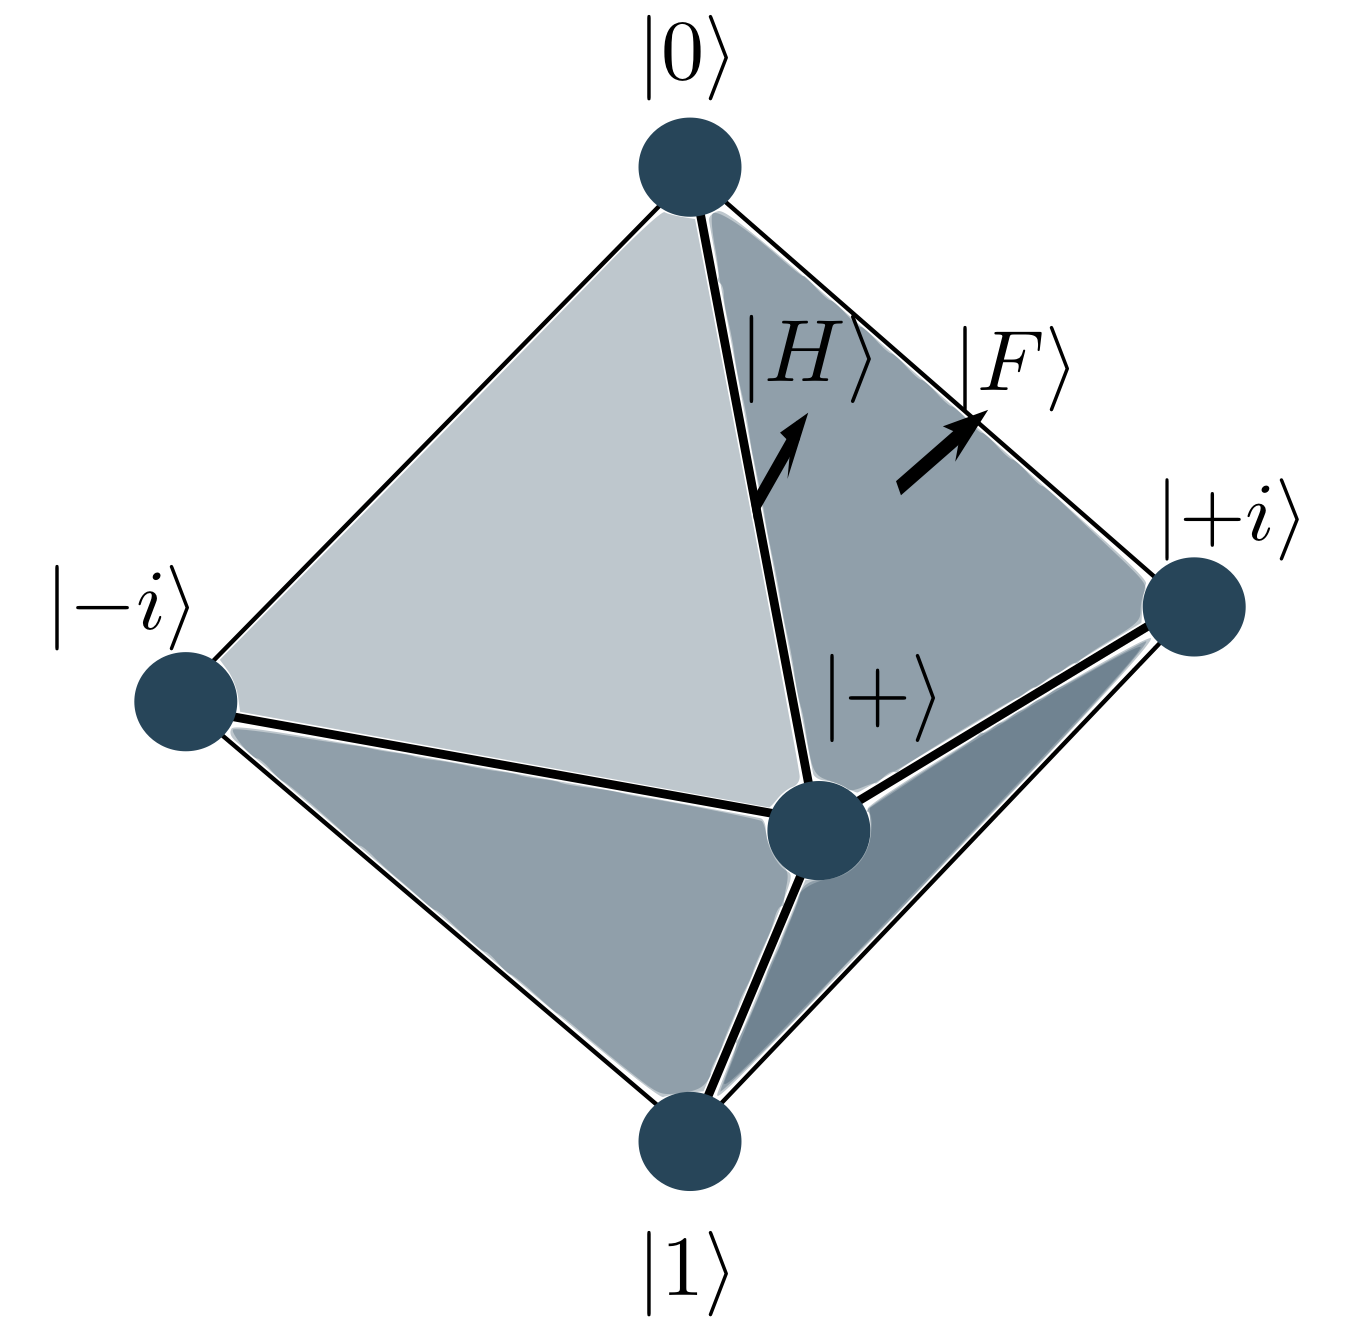
\includegraphics[width=0.5\textwidth]{octahedron.png}
\caption{Diagram showing the location of single-qubit stabilizer states and magic states on the Bloch sphere. Single qubit Clifford gates act as the symmetry group of an octahedron in the Bloch sphere, who's vertices are the individual stabilizer states. `Edge' and `face' magic states are named for their positions relative to this octahedron. Based on diagrams given in from~\cite{Bravyi2005}.}
\end{figure}
We further examined the stabilizer rank for different quantum states by extending the computational searches of~\cite{Bravyi2015}.
\subsubsection*{Computation Searches for Decompositions}
We employ a combination of brute force and random walk searches for stabilizer state decompositions to establish the stabilizer rank of different families of quantum states, using a custom program developed in Python.\par
To test a candidate decomposition of $\chi$ stabilizer states $\Phi=\{\ket{\phi_{i}}\}$, we compute the projector on to the subspace generated by the states $\Pi_{\Phi}$, and the compute the projection of the target state into this subspace $\norm{\Pi_{\Phi}\ket{\psi}}$. If the norm is equal to $1$, then the state lies within this subspace and we terminate the search.\par
Given a collection of $\chi$ stabilizer states, we can build their projector by first constructing a $2^{n}\times \chi$ matrix $A$ where each column is one of the $\chi$ stabilizer states. We then apply the QR decomposition, a standard linear algebra technique, to compute $\chi$ orthogonal basis-vectors for the subspace spanned by these stabilizer states. Given the column matrix $Q$ built from these orthogonal basis-vectors, we then have $\Pi_{\Phi}\equiv Q\,Q^{\dagger}$. This was implemented using the \texttt{Numpy} library, with additional optimization provided by using the \texttt{Numba} Just-In-Time compiler~\cite{Numpy,Numba}.\par
The random walk method follows the description in Appendix~B of~\cite{Bravyi2015}. The search algorithm takes as input a state $\ket{\psi}$ to decompose, and a candidate stabilizer rank $\chi$. We begin with a candidate decomposition $\Phi=\{\ket{\phi_{i}}\}$, and compute the `distance' from the generated subspace $F=1-\norm{\Pi_{\Phi}\ket{\psi}}$. We then update one state, chosen uniformly at random, by applying a random Pauli operator $P$. We then compute the updated distance $F'=1-\norm{\Pi_{\tilde{\Phi}}\ket{\psi}}$ using this updated set of stabilizer states. If $F'<F$, we accept the move and proceed. Otherwise, we accept the move with a probability given by the Boltzmann distribution $p=\mathe^{-\beta\left(F'-F\right)}$, where $\beta$ is a parameter we set. As the search continues, we gradually increase $\beta$. This method is thus similar to the simulated annealing approach in optimization, where we are seeking to minimize the distance between $\ket{\psi}$ and the generated subspace.\par
Our random walks were run using the same parameters of~\cite{Bravyi2015}, testing $100$ values of the inverse-temperature parameter $\beta\in [100,4000]$, and running for $1000$ steps for each value of $\beta$. For any given candidate and value of $\chi$, we repeated the random walk $5$ times. The smallest decomposition found across all runs was taken as an upper bound on the stabilizer rank. As with the brute force searches, $\chi=2$ was taken as a lower bound, and the largest value tested was either $2^{n}-1$, or else a value derived using submultiplicativity and results for fewer copies of the target state.\par
The brute force method, in contrast, takes as input a target state $\ket{\psi}$, and an upper and lower bound of stabilizer rank to test. The typical lower bound given is $2$. The upper-bound is set by either the computational basis expansion, which is a valid stabilizer state decomposition, or else a bound based on submultiplicativity and known results for fewer copies of a state.\par
Pseudocode descriptions of the search methods are given in Algorithms~\ref{alg:random_walk} and~\ref{alg:brute_force}. We also note an additional optimisation that, in the case where the target state has only real coefficients, we can restrict ourselves to considering decompositions built only from stabilizer states with real values. In the random walk case, we additionally restrict the moves we generate such that they do not introduce any imaginary coefficients. We do this by requiring that the random Pauli operators have an even number of Pauli $Y$ operators.\par
As mentioned above, the number of stabilizer states grows exponentially with the number of qubits. In particular, we have~\cite{Aaronson2004}
\begin{equation}
N_{\phi} = 2^{n}\prod_{k=1}^{n-1}\left(2^{n-k}+1\right).
\end{equation}
In practice, brute force searches were tractable up to about $3$ qubits. Some examples of the growth in possible combinations are given in Table~\ref{tab:n_combinations}.\par
\begin{table}[H]
\centering
\begin{tabular}{| l | c | c | c | c |}
\hline
$n$ Qubits & $1$ & $2$ & $3$ & $4$ \\ \hline
$N_{\phi}$ & $6$ & $60$ & $1080$ & $36720$ \\ \hline
$\binom{N_{\phi}}{2^{n}-1}$ & $6$ & $33240$ & $3.33\times10^{17}$ & $2.27\times 10^{56}$ \\ \hline
\end{tabular}
\caption{Table showing how the number of combinations of stabilizer states grows as a function for the number of qubits. We consider $2^{n}-1$ as this is the largest possible stabilizer rank that is below the trivial computational basis bound.}
\label{tab:n_combinations}
\end{table}
\begin{algorithm}[p]
\caption{Random Walk Search for Stabilizer State Decomposition}
\label{alg:random_walk}
\begin{algorithmic}[1]
\Require $\beta_{init},\beta_{max},M$, target integer $\chi$
\Require \Call{Projector}{$\Phi$} \Comment{Returns projector onto subspace spanned by $\Phi$}
\State $\Phi \leftarrow \left(\phi_{1},\cdots\phi_{\chi}\right)$ where each $\phi_{a}$ is chosen at random.
\State $\beta \leftarrow \beta_{init}$
\While{$\beta < \beta_{max}$}
    \For{$i=0$ to $1000$}
        \State $\Pi_{\Phi}\gets$\Call{Projector}{$\Phi$}
        \State $F(\tilde{\phi})= 1-\norm{\Pi_{\phi}\ket{\psi}}$
        \If{$F(\tilde{\phi})=1$}
            \State \Return $\tilde{\phi}$
        \EndIf
        \State Pick random integer $a\in[1,n]$ and random Pauli $P\in\mathcal{P}_{n}$
        \State $\ket{\phi_{a}}'\leftarrow c\left(\mathbb{I}+P\right)\ket{\phi_{a}}$ \Comment{If $\ket{\phi_{a}}'=0$, pick new $a$ and $P$.}
        \State $\tilde{\Phi} \leftarrow (\ket{\phi_{1}},\cdots,\ket{\phi_{a}}',\cdots\ket{\phi_{\chi}})$
        \State $\Pi_{\tilde{\Phi}}\gets$\Call{Projector}{$\tilde{\Phi}$}
        \State $F'\gets 1-\norm{\Pi_{\tilde{\Phi}}\ket{\psi}}$
        \If{$F'<F$}
            \State $\ket{\phi_{a}}\leftarrow \ket{\phi_{a}}'$
        \Else
            \State $p_{accept}\leftarrow \exp[-\beta\left(F'-F\right)]$
            \State Pick random $r\in [0,1]$
            \If{$r<p_{accept}$}
                \State $\ket{\phi_{a}}\leftarrow \ket{\phi_{a}}'$
            \EndIf
        \EndIf
    \EndFor
    \State $\beta\leftarrow \beta + \left( \frac{\beta_{\mathrm{max}}-\beta_{\mathrm{init}} }{M} \right)$
\EndWhile
\State \Return No decomposition found.
\end{algorithmic}
\end{algorithm}
\begin{algorithm}[p]
\caption{Brute Force Search for stabilizer rank}
\label{alg:brute_force}
\begin{algorithmic}[1]
    \Require $\{\phi\}_{n}$ \Comment{The set of $n$ qubit stabilizer states}
    \Require \Call{Projector}{$\Phi$} \Comment{Returns projector onto subspace spanned by $\Phi$.}
    \State $\chi=2$
    \While{$\chi<\left(2^{n}-1\right)$}
        \For $\Phi=\{\ket{phi_{1}},\dots,\ket{\phi_{\chi}}$ \Comment{For all combinations of $i$ states.}
            \State $\Pi_{\Phi}\leftarrow$ \Call{Projector}{$\Phi$}
            \If{$\norm{\Pi_{\tilde{\Phi}}\ket{\psi}}$ = $1$}
                \State \Return $\chi,\Phi$
            \EndIf
        \EndFor
    \State $\chi\leftarrow \chi+1$
    \EndWhile
    \State \Return $2^{n}$ \Comment{The computational basis expansion is the best found.}
\end{algorithmic}
\end{algorithm}
\par\large{\itshape{Generating Stabilizer States}}\par
As an input for Algorithms~\ref{alg:random_walk} and~\ref{alg:brute_force}, we need a way to quickly generate random stabilizer states, as well as a library of all stabilizer states for small $n$. To accomplish this, we make use of the canonical form for stabilizer tableaux introduced by Garcia et al., and discussed in Section~\ref{sec:stabilizer-intro}~\cite{Garcia2012}.\par
Like the CHP method, a canonical stabilizer tableau is a $n \times \left(2n+1\right)$ matrix, where each row encodes a Pauli operator
\[P\left(s\right)=-1^{s_{0}}\otimes_{i=1}^{n}X^{s_{i}}Z^{s_{i+n}},\;:\;s\in\mathbb{Z}_{2}^{2n+1}.\]
There are in general multiple tableau corresponding to a given stabilizer state, but using Algorithm~1 of~\cite{Garcia2012} any tableau can be converted to a standard form.\par
To quickly generate random stabilizer states then, we generate a random $n \times \left(2n+1\right)$ binary matrix. We then apply the canonical form algorithm. If any rows of the tableau are the all-$0$ string, then the tableau does not correspond to a stabilizer state and so we discard it. Else, we build up a Pauli projector from the rows of the tableau, and compute the stabilizer state as the unique $+1$ eigenstate.\par
To generate a complete library of stabilizer states, first recall that Pauli operators in a stabilizer group have only phase of $\pm 1$. For a stabilizer group with $n$ generators, there are thus $2^{n}$ possible combinations of phase for each generator, each of which correspond to a given stabilizer state. We can thus focus on generating just the $N_{\phi}/2^{n}$ stabilizer groups with all positive phase.\par
We begin by generating all $2^{2n}-1$ possible binary strings, which correspond to all possible choices of Pauli operator. We ignore the all $0$ string, as this corresponds to the identity operator which cannot generate a stabilizer group. Then, for all $\binom{2^{2n}-1}{n}$ possible combinations of $n$ strings, we build the stabilizer tableau and convert it to canonical form. If it is not full rank, or corresponds to a tableau already found, we discard it. Otherwise we store the tableau. We terminate after generating $N_{\phi}/2^{n}$ groups. For each group then, we test all $2^{n}$ possible phase combinations, and then compute the stabilizer state as described above. This process was quite computationally intensive, but overall we were able to generate a library of stabilizer states on up to $4$ qubits.\par
Both the random stabilizer state generation and the deterministic stabilizer state generation were implemented in Python. Stabilizer tableau were stored as bitpacked \texttt{Numpy} arrays. Computing the corresponding Pauli projector and stabilizer state made use of \texttt{Numpy} linear algebra routines, including the optimised eigensovler for hermitian matrices, with additional optimization using \texttt{Numba}~\cite{Numpy,Numba}.
\subsubsection*{Results of Computational Searches}
We extend the computational searches for copies of single-qubit magic states up to $n=10$, and give explicit results for the face-type magic states. We used brute force searches for $n\leq 3$ qubits. Otherwise, we made use of random walk searches. 
\par
For all values of $n$ tested, the edge and face type magic states had the same observed stabilizer rank. Despite extending the range of the numeric search, however, above $n=6$ copies we found no decomposition smaller than the submultiplicative bound. Thus, the asymptotic scaling shown in~\cite{Bravyi2015} remains the best result known for single-qubit magic states..\par
As a means of probing Conjecture~\ref{conj:magic_srank}, we also explored the stabilizer rank of `typical' single qubit states, generated uniformly at random. The target states were prepared by applying a Haar random single-qubit unitary to the $\ket{0}$ states~\cite{Lundberg2004}. We began by applying brute force searches to $1000$ typical states up to $3$ copies, and observed that all states tested had the same stabilizer rank, and also that their stabilizer rank grew more slowly than the computational basis expansion. All results for single qubit states are shown in Table~\ref{tab:exact_rank_results}.\par
Applying the argument of Eq.~\ref{eq:exact_t_state_bound}, then for typical single qubit states their stabilizer rank is upper bounded by
\begin{equation}
\chi\left(\ket{\phi^{\otimes t}}\right)\leq 8^{t/6}=2^{\log_{2}{8}t/6}=2^{0.5t}.
\label{eq:typical_state_srank}
\end{equation}
To further explore the claim in Conjecture~\ref{conj:magic_srank}, we also performed computational searches for specific states with a structure related to the magic states. In particular, we performed computational searches for the $\ket{CS}$ and $\ket{CCZ}$ magic states, which can be used to inject the two-qubit $CS$ gate and the three-qubit $CCZ$ gate, respectively. Both of these gates, like the $T$ gate, belong to the third level of the Clifford hierarchy. We also considered the single qubit resource states $T^{\frac{1}{2}}\ket{+}$ and $T^{\frac{1}{4}}\ket{+}$. These resource states can be used to inject gates from the $4$th and $5$th levels of the Clifford hierarchy, though potentially requiring a non-Clifford correction operation. We limited our searches up to $6$ qubits, which meant considering up to $3$ copies of the $\ket{CS}$ state and just two copies of the $CCZ$ state The results are show in table~\ref{tab:resource_state_rank}.\par
Interestingly, we observe that the single qubit resource states corresponding to gates in higher levels of the Clifford hierarchy show no difference from the stabilizer rank of typical single qubit states. However, magic states on $2$ and $3$ qubits also show significantly reduced stabilizer rank. In fact, the asymptotic scaling of the $\ket{CS}$ and $\ket{CCZ}$ is significantly smaller when compared to the naive computational basis expansion, scaling as $\approx 2^{0.79  t}$ and $2^{t}$ versus $2^{2t}$ and $2^{3t}$, respectively.
\begin{table}[H]
\centering
\begin{tabular}{|l|c|c|c|c|c|c|c|c|c|}
\hline
$t$ Copies & 2 & 3 & 4 & 5 & 6 & 7 & 8 & 9 & 10\\ \hline
$\chi\left(\ket{T^{\otimes t}}\right)$ & 2 & 3 & 4 & 6 & 7 & 12 & 14 & 21 & 28 \\ 
$\chi\left(\ket{F^{\otimes t}}\right)$ & 2 & 3 & 4 & 6 & 7 & 12 & 14 & 21 & 28 \\ 
$\chi\left(\text{Typical}\right)$ & 3 & 4 & 5 & 6 & 8 & 14 & 24 & 30 & 36 \\ \hline
\end{tabular}
\caption{Results of computational searches for stabilizer rank decompositions of different single-qubit quantum states. The results would appear to agree with Conjecture~\ref{conj:magic_srank}, that stabilizer rank is smaller for magic states.}
\label{tab:exact_rank_results}
\end{table}
\begin{table}[H]
\centering
\begin{tabular}{|l|c|c|c|c|}
\hline
$t$ Copies & 1 & 2 & 3 & 4 \\ \hline
$T^{\frac{1}{2}}\ket{+}$ & 2 & 3 & 4 & 5 \\
$T^{\frac{1}{4}}\ket{+}$ & 2 & 3 & 4 & 5 \\
$\ket{CS}$ & 2 & 3 & 6 & - \\
$\ket{CCZ}$ & 2 & 4 & - & - \\ \hline
\end{tabular}
\caption{Results of computational searches for stabilizer rank decompositions of different types of non-stabilizer resource state. We extended the searches for the $T^{\frac{1}{2}}$ and $T^{\frac{1}{4}}$ gate resource states up to $6$ copies, but found no decompositions smaller than the results for typical single qubit states.}
\label{tab:resource_state_rank}
\end{table}
\par
\large{\itshape{Decompositions of the Symmetric Subspace}}\par
When taking multiple copies of any given $n$-qubit state $\ket{\psi}$, the result will always lie within the symmetric subspace $\text{Sym}_{n,t}\subseteq \mathbb{C}^{2^{n}}$. This is a subspace of the full $n$-qubit Hilbert space with dimension
\begin{equation}
\text{dim}\left( \text{Sym}_{n,t}\right ) = \binom{2^{n}+t-1}{t}
\end{equation}
We can thus consider searching for stabilizer state decompositions of a subspace. We define the exact stabilizer rank of a subspace $P$ as
\begin{equation}
\chi\left(P\right) = \left| \Phi\right| : P\in \text{span}[\Phi].
\label{eq:subspace_srank}
\end{equation}
Computationally, we employ the Random Walk method, to build decompositions of the subspace $\text{Sym}_{1,t}$. As our objective function, we replace the projection into the subspace $\Pi_{\Phi}$ with the largest principle angle between two subspaces $\Pi_{\Phi}$ and $\Pi_{\text{Sym}_{1,t}}$. If $\text{Sym}_{1,t}\subseteq\text{Span}\left(\Phi\right)$, this angle is zero. The formula for the largest principle angle is shown in Eq.~\ref{eq:subspace_angle}~\cite{Knyazev2002}. The projector onto the symmetric subspace, $\Pi_{\text{Sym}_{1,t}}$, was computed using the method based on superpositions of computational basis states with equal Hamming weight, outlined in~\cite{Harrow2013}.\par
\begin{equation}
\theta\left(\Pi_{\Phi},\Pi_{\text{Sym}_{1,t}}\right)=\sin^{-1}\left(\norm{\left(I-\Pi_{\Phi}\right)\Pi_{\text{Syn}_{1,t}}}\right)
\label{eq:subspace_angle}
\end{equation}
For all values tested, the best decomposition found for the projector onto the single qubit symmetric subspace were equal to the results for typical single qubit states. Additionally, we note that for $t\leq 5$
\begin{equation}
\chi\left(\text{Sym}_{1,t}\right) = \text{dim}\left( \text{Sym}_{1,t}\right) \leq t+1 = \binom{2+t-1}{t},
\end{equation}
the stabilizer rank found for the single qubit symmetric subspace is equal to its dimension.\par
In fact, in~\cite{Bravyi2018}, we make the following claim
\begin{cla}
$\chi\left(\text{Sym}_{n,t}\right)=\text{dim}\left(\text{Sym}_{n,t}\right)\,:\forall n,\; t\leq 5$\label{cla:symmetric_srank}
\end{cla}
For $t\leq 3$, this claim follows from the property that stabilizer states form a projective $3$ design~\cite{Zhu2016}. Thus, for a given $n$ qubits and $t\leq 3$
\begin{equation}
\frac{1}{N_{\phi}}\sum_{i}\ketbra{\phi_{i}}=\frac{\Pi_{\text{Sym}_{n,t}}}{\text{dim}\left(\text{Sym}_{n,t}\right)},
\end{equation}
a superposition of $t$ copies of all $n$-qubit stabilizer states is proportional to the projector onto the symmetric subspace.\par
From this, we can conclude that $\text{Span}\left(\left\{\ket{\phi_{i}^{\otimes t}}\right\}\right)\subseteq \Pi_{\text{Sym}_{n,t}}$. We can thus find a minimal spanning set of vectors $\{\ket{\phi_{j}^{\otimes t}}\}$ such that $\text{Span}\left(\{\ket{\phi_{j}^{\otimes t}}\}\right)=\text{Sym}_{n,t}$, and $\left|\{\ket{\phi_{j}^{\otimes t}}\}\right|=\text{dim}\left(\text{Sym}_{n,t}\right)$, completing the claim for $t\leq 3$. In~\cite{Bravyi2018}, we present a proof by Earl Campbell that also extends this result up to $t=5$ using the fact that stabilizer states are `almost' a projective $4$-design~\cite{Zhu2016}.
\subsubsection*{Clifford Symmetries}
The results of computational searches, and the proof for the decomposition of the symmetric subspace, are consistent with Conjecture~\ref{conj:magic_srank}. In Table~\ref{tab:srank_tables}, we compare the bounds for the symmetric subspace with the stabilizer rank decompositions found for different magic states, and show that in general the magic states exhibit a smaller stabilizer rank.\par
\begin{table}[H]
\centering
    \begin{subtable}[t]{0.6\textwidth}
    \caption{}
    \centering
        \begin{tabular}{|l|c|c|c|c|}
            \hline
            $n$ Copies & 2 & 3 & 4 & 5 \\
            \hline
            $\text{dim}\left(\text{Sym}_{n,t}\right)$ & 3 & 4 & 5 & 6 \\
            $\chi\left(\ket{T,F}\right)$ & 2 & 3 & 4 & 6 \\ \hline
        \end{tabular}
    \end{subtable}
    \vspace{1cm}
    \begin{subtable}[t]{0.48\textwidth}
    \centering
        \begin{tabular}{|l|c|c|c|}
            \hline
            $n$ Copies & 1 & 2 & 3 \\ \hline
            $\text{dim}\left(\text{Sym}_{n,t}\right)$ & 4 & 10 & 20 \\
            $\chi\left(\ket{CS}\right)$ & 2 & 3 & 6 \\ \hline
        \end{tabular}
        \caption{}
    \end{subtable}
    \begin{subtable}[t]{0.48\textwidth}
    \centering
        \begin{tabular}{|l|c|c|}
            \hline
            $n$ Copies & 1 & 2 \\ \hline
            $\text{dim}\left(\text{Sym}_{n,t}\right)$ & 8 & 36 \\
            $\ket{CCZ}$ & 2 & 4 \\ \hline
        \end{tabular}
        \caption{}
    \end{subtable}
    \caption{Tables comparing the dimension, and thus stabilizer rank, of the symmetric subspace up to $5$ copies with that of magic states, for $1$, $2$ and $3$ qubits.}
\label{tab:srank_tables}
\end{table}
A property common to all the magic states tested is that they each have an associated Clifford symmetry. This is in fact always true for a magic state that can be used to inject a gate from $\mathcal{C}_{3}$. These magic states have the form $\ket{U}=U\ket{\phi}$, where $\ket{\phi}$ is a stabilizer state~\cite{Gottesman1999}. Updating the stabilizer group under conjugation, we obtain a new set of operators that stabilizer the resource state $\ket{U}$
\begin{equation}
S\ket{\phi} =\ket{\phi} \rightarrow USU^{\dagger} \ket{U} = USU^{\dagger}U\ket{\phi} = U\ket{\phi}\;\forall S\in\mathcal{S}_{\phi}.
\end{equation}
From the definition of $\mathcal{C}_{3}$, these operators are then Clifford as $USU^{\dagger}\in\mathcal{C}_{2}$, and also form a group which we call $\mathcal{M}$. We introduce the following nomenclature.
\begin{defn}[Clifford Magic State]
Consider a magic state $\ket{R}$, with an associated group of Clifford symmetries $\mathcal{M}$ such that
\begin{enumerate}
    \item $\mathcal{M}\subseteq \mathcal{C}_{2}$
    \item $m\ket{R} =\ket{R}\;\forall\,m\in\mathcal{M}$
    \item $\ketbra{R}=\frac{1}{\left|\mathcal{M}\right|} \sum_{m\in\mathcal{M}} m $
\end{enumerate}
Then $\ket{R}$ is a Clifford magic state.\footnote{Note that this differs from the definition in~\cite{Bravyi2018}. We introduce this definition in this thesis as we consider slightly broader classes of magic state which nonetheless share the property of Clifford symmetries.}
\end{defn}
Any state that can be consumed in a state-injection gadget is also a Clifford magic state.. For example, the $\ket{H}$ magic state is so labeled as it has the property that $H\ket{H}=\ket{H}$, and thus has the group $\{I,H\}$ as its Clifford symmetry. We note however that the face-type magic states are also Clifford magic states. The state $\ket{F}$, for example, is fixed by a group generated by the Clifford gate $F$. The $F$ gate corresponds to a rotational symmetry of the faces of the stabilizer octahedron, as can be seen by its action on the single qubit stabilizer states.
\begin{equation}
\begin{array}{l c r}
F \ket{0}=\ket{+} & F\ket{+i} = \ket{+} & F\ket{+} = 0
\end{array}
\end{equation}
It was shown by Earl Campbell that quotient groups of Clifford symmetries can be used to find the stabilizer rank of Clifford magic states $\ket{R}$. 
\begin{lem}\label{lem:quotient_srank}
Consider a stabilizer state $\ket{\phi_{0}}:\braket{\phi_{0}}{\psi}\neq 0$. We will denote by $\mathcal{M}$ the group of Clifford symmetries of $\ket{\phi}$. Let $\mathcal{N}\subseteq\mathcal{M}$ be the subgroup of $\mathcal{M}$ such that $n\ket{\phi_{0}}=\ket{\phi_{0}}\forall n\in\mathcal{N}$, and define $\mathcal{Q}$ as the quotient group $\mathcal{M}/\mathcal{N}$. Then
\begin{equation}
\chi\left(\ket{\phi}\right)\leq \frac{\left|\mathcal{M}\right|}{\left|\mathcal{M}\right|}
\label{eq:quotient_srank}
\end{equation}
with stabilizer state decomposition
\begin{equation}
\ket{\psi} \propto \sum_{q\in\mathcal{Q}}q\ket{\phi_{0}}
\label{eq:subgroup_decomposition}
\end{equation}
\end{lem}
\begin{proof}[Proof of Lemma~\ref{lem:quotient_srank}]
We can expand out $\ket{\phi_{0}}$ as
\[\ket{\phi_{0}}=\frac{1}{\left|\mathcal{N}\right|}\sum_{n\in\mathcal{N}}n\ket{\phi_{0}}.\]
Making this substitution for $\ket{\phi_{0}}$, we thus have
\begin{align*}
\sum_{q\in\mathcal{Q}}q\ket{\phi_{0}}&=\sum_{q\in\mathcal{Q}}\sum_{n\in\mathcal{N}}qn\ket{\phi_{0}}\\&=\sum_{m\in\mathcal{M}}m\ket{\phi_{0}}
\end{align*}
where on the last line we use the definition of the quotient group. From the definition of $\mathcal{M}$, we can write
\[\sum_{m\in\mathcal{M}}=\braket{\psi}\]
and thus
\begin{align*}
\sum_{q}q\ket{\phi_{0}}&=\frac{\left|\mathcal{M}\right|}{\left|\mathcal{N}\right|} \ket{\psi}\braket{\psi}{\phi_{0}}\\
\implies \ket{\psi} &= \frac{\left|\mathcal{N}\right|}{\left|\mathcal{M}\right|\braket{\psi}{\phi_{0}}} \sum_{q\in\mathcal{Q}}q\ket{\phi_{0}}
\end{align*}
completing the proof.
\end{proof}
As an example, consider the state $\ket{H^{\otimes 2}}$. This state has the Clifford symmetry group $\{I, H\otimes I, I\otimes H, H\otimes H\}$. We can build a $2$-element normal subgroup $\{I,H\otimes H\}$, which stabilizes the state $
\ket{0}\ket{+} + \ket{1}\ket{-}$. This give a stabilizer rank of $\left|\mathcal{M}\right|/\left|\mathcal{N}\right|=\frac{4}{2}=2$, as expected.\par
One interesting extension of this result is that any resource state used to inject controlled diagonal Clifford gate, such as $CCZ$ or $CS$, also has a stabilizer rank of $2$, which agrees with the results of the computational searches in Table~\ref{tab:srank_tables}. The stabilizer state decompositions for these states can in fact be found by considering the resource state itself. Expanding out the action of the control, we have
\begin{equation}
U\equiv \ketbra{0}\otimes I+\ketbra{1}\otimes C \implies U\ket{+^{\otimes n}}\propto \ket{0}\ket{+}^{\otimes n-1}+\ket{1}C\ket{+^{\otimes n-1}}
\end{equation}
which is a stabilizer state decomposition with $\chi=2$ as $C$ is a Clifford operator, and thus $C\ket{+^{\otimes n-1}}$ is a stabilizer state.\par
However, here we show that this method does not always produce optimal stabilizer state decompositions. For example, consider the $\ket{F}$ state. A single copy has Clifford symmetry group $\{I, F, F^{2}\}$, which has no non-trivial subgroups. This would suggest $\chi\left(\ket{F}\right)\leq 3$, which is larger than just the computational basis bound.\par
For two copies, $|ket{F^{\otimes 2}}$ has the 9-element symmetry group
\begin{equation}
\{I,FI, IF, F^{2}I, IF^{2}, FF, F^{2}F, FF^{2}, F^{2}F^{2}\},
\label{eq:f2_symmetry_group}
\end{equation} where we omit the tensor product symbol for brevity. From the Lagrange theorem, we know that the order of any subgroup $\mathcal{N}\subseteq\mathcal{M}$ must divide the order of the group~\cite{Artin2010}. Thus, the smallest possible quotient group has $\left|\mathcal{Q}\right|=3$. Again, this is larger than the known optimal decomposition $\chi\left(\ket{F^{\otimes 2}}\right)=2$.\par
We can further consider extending this method to include permutation symmetries. For $t$ copies of single qubit states, the permutation symmetries correspond to the symmetric group $S(t)$, and can be generated using swap permutations~\cite{Artin2010}. In terms of quantum gates, these permutations correspond to the $SWAP$ gate, which is a Clifford operator as it can be realised by a sequence of $3$ $CNOT$ gates.\par
Extending the groups to incorporate these permutation symmetries allows us to generate subgroups with the correct index. For example, for the $\ket{H^{\otimes 2}}$ state, incorporating permutations gives an order $8$ symmetry group, with a subgroup of order $4$ and thus index $2$. This subgroup $\mathcal{N}=\{I, SWAP, HH, SWAP\,HH\}$, fixes the same stabilizer state $\ket{0}\ket{+}+\ket{1}\ket{-}$, and thus we again have $\chi=2$.\par
Similarly, for the $\ket{F^{\otimes 2}}$ state, we obtain an order $18$ Clifford symmetry group by incorporating permutations, and can construct a subgroup of order $9$ and thus index $2$. However, this subgroup $\mathcal{N}$ corresponds to the group given in Eq.~\ref{eq:f2_symmetry_group}, which fixes the state $\ket{F^{\otimes 2}}$. Thus, there is no stabilizer state $\ket{\phi_{0}}:n\ket{\phi_{0}}=\ket{\phi_{0}}\;\forall\,n\in\mathcal{N}$, and we cannot use this result to build a stabilizer state decomposition.
\subsection{Approximate Stabilizer Rank}\label{sec:approx_results}
% Outline rough idea of taking decomposition and approximating it
In this section, we show how to construct approximate stabilizer state decompositions for Clifford magic states, and more generally. Both methods start with an exact stabilizer state decomposition, which is not required to be optimal, and show how to construct an approximate decomposition by discarding terms.
\subsubsection*{Clifford Magic States}
A method for constructing approximate stabilizer state decompositions of the $\ket{H}$ magic state was described in~\cite{Bravyi2016}. Here, we outline their argument, showing how it can naturally be extended to any Clifford magic state, such as $\ket{F}$ or $\ket{CCZ}$.\par
The authors begin by considering an exact stabilizer state decomposition of $\ket{H^{\otimes t}}$ in terms of the states $\ket{0}$ and $\ket{+}$.
\begin{equation}
\ket{H^{\otimes t}} = \frac{1}{2\cos\left(\pi/8\right)^{t}}\sum_{\tilde{x}\in\mathbb{Z}_{2}^{t}} \ket{x}
\label{eq:exact_H_expansion}
\end{equation}
where $\ket{\tilde{x}}$ is a $t$-qubit state such that
\begin{equation}
\ket{\tilde{x}}=\otimes_{i=1}^{t} H^{\tilde{x}_{i}}\ket{0}
\label{eq:xtilde_bits}.
\end{equation}
Each term in the decomposition is a tensor product of stabilizer states, generated by a subgroup of the Clifford group. Recalling Eq.~\ref{eq:subgroup_decomposition}, we can construct a stabilizer state decomposition for a Clifford magic state $\ket{R}$ from a group $\mathcal{Q}\subseteq \mathcal{C}_{2}$, and a state $\ket{\phi_{0}}\,:\,\braket{\phi_{0}}{R}>0$. We can write
\[\ket{R}\propto \sum_{q\in\mathcal{Q}}\ket{\phi_{q}} \;:\,\ket{\phi_{q}}=q\ket{\phi_{0}}.\]
To normalize the decomposition, we note that $\braket{\phi_{q}}{R}=\matrixel{\phi_{0}}{q^{-1}}{R}=\braket{\phi_{0}}{R}$. Thus, 
\begin{align}
\ket{R}& =\frac{1}{\left|Q\right|\braket{\phi_{0}}{R}}\sum_{q\in\mathcal{Q}}\ket{\phi_{q}} \nonumber \\
\implies \ket{R}^{\otimes t}&=\frac{1}{\left(\left|\mathcal{Q}\right|\braket{\phi_{0}}{R}\right)^{t}}\sum_{\va{q}\in\mathbb{Z}_{\left|\mathcal{Q}\right|}^{t}}\ket{\phi_{\va{q}}}
\label{eq:clifford_sym_decomposition}
\end{align}
where $\ket{\phi}_{\va{q}}\equiv\otimes_{i=1}^{t}\ket{\phi_{\va{q}_{i}}}$ and $\va{q}$ is $t$-element vector where each entry denotes a member of the group. Setting $\left|\mathcal{Q}\right|=2$ and $\ket{\phi_{0}}=\ket{0}$, gives the same decomposition for $\ket{H^{\otimes t}}$ given in Eq.~\ref{eq:exact_H_expansion}.\par
We can also define states $\ket{\mathcal{L}}$, built from subspaces $\mathcal{L}\subseteq\mathbb{Z}_{\left|\mathcal{Q}\right|}^{t}$
\begin{equation}
\ket{\mathcal{L}} = \frac{1}{\sqrt{\left|\mathcal{L}\right|Z\left(\mathcal{L}\right)}}\sum_{\va{q}\in\mathcal{L}}\ket{\phi_{\va{q}}},
\label{eq:weight}
\end{equation}
where $\left|\mathcal{L}\right|$ is the number of elements in the subspace, and $Z\left(\mathcal{L}\right)$ is a normalisation factor, given by
\begin{align*}
\braket{\mathcal{L}}=1 &=\frac{1}{\left|\mathcal{L}\right|Z\left(\mathcal{L}\right)}\sum_{\va{p},\va{q}\in\mathcal{L}}\braket{\phi_{p}}{\phi_{q}} \nonumber \\
&=\frac{1}{\left|\mathcal{L}\right|Z\left(\mathcal{L}\right)}\sum_{\va{p}\va{q}}\braket{\phi_{\va{0}}}{\phi_{\va{p}^{-1}\va{q}}} \nonumber \\
&=\frac{1}{Z\left(\mathcal{L}\right)}\sum_{\va{q}}\braket{\phi_{\va{0}}}{\phi_{\va{q}}}
\end{align*}
where in the last line we have used the group properties of $\mathcal{Q}$ to simplify the sum, and where $\ket{\phi_{\va{0}}}=\ket{\phi_{0}^{\otimes t}}$.\par
How well does a given subspace with $\left|\mathcal{L}\right|<2^{t}$ approximate the full stabilizer state decomposition? Each term in the subspace state has overlap $\left(\braket{\phi_{0}}{R}\right)^{t}$, and thus
\begin{equation}
\left|\braket{R^{\otimes t}}{\mathcal{L}}\right|^{2}
=
\frac{\left|\mathcal{L}\right|^{2}f_{\phi_{0}}^{t}\left(R\right)}{\left|\mathcal{L}\right|Z\left(\mathcal{L}\right)}=\frac{\left|\mathcal{L}\right|f_{\phi_{0}}\left(R\right)}{Z\left(\mathcal{L}\right)}
\label{eq:incomplete_r_fidelity}
\end{equation}
where we define $f_{\phi_{0}}\left(R\right)\equiv\left|\braket{\phi_{0}}{R}\right|^{2}$, the fidelity of $\ket{\phi_{0}}$ with $\ket{R}$.\par
The fidelity of the $\mathcal{L}$ approximate thus depends on the size of the subspace, the initial overlap, and the quantity $Z\left(\mathcal{L}\right)$ which depends on the subspace we choose. Bravyi \& Gosset then showed for the case of the $\ket{H}$ state that we can achieve $Z\left(\mathcal{L}\right)\sim 1+\left|\mathcal{L}\right|f_{\phi_{0}}\left(H\right)^{t}$ by choosing subspaces at random~\cite{Bravyi2016}.\par
This argument also extends to the more general case of Clifford symmetries. Choosing subspaces uniformly at random, we can compute the expectation value of the weight $Z\left(\mathcal{L}\right)$. Every subspace must contain $\ket{\phi_{\va{0}}}$, which contributes $\braket{\phi_{\va{0}}}=1$ to the weight. Otherwise, each state $\ket{\phi_{\va{q}}}$ is equiprobable, and occurs with probability $\frac{\left|\mathcal{L}-1\right|}{\left|Q\right|^{t}-1}$. Thus,
\begin{equation}
\mathbb{E}\left[Z\left(\mathcal{L}\right)\right] = 1 + \frac{\left|\mathcal{L}\right|-1}{\left|Q\right|^{t}-1}\left(\sum_{\va{q}\in\mathbb{Z}_{\left|\mathcal{Q}\right|}^{t}-1}\braket{\phi_{\va{q}}}{\phi_{\va{0}}}\right).
\end{equation}
By replacing $\sum_{\va{q}\in\mathbb{Z}_{\left|\mathcal{Q}\right|}^{t}-1}\braket{\phi_{\va{q}}}{\phi_{\va{0}}}$ with $\sum_{\va{q}\in\mathbb{Z}_{\left|\mathcal{Q}\right|}^{t}}\braket{\phi_{\va{q}}}{\phi_{\va{0}}} -1$, and substituting Eq.~\ref{eq:clifford_sym_decomposition}, we can write
\begin{equation}
\mathbb{E}\left[Z\left(\mathcal{L}\right)\right] = 1 + \frac{\left|\mathcal{L}\right|-1}{\left|Q\right|^{t}-1}\left(\left|\mathcal{Q}\right|^{t}f_{\phi_{0}}\left(R\right)-1\right)\approx 1+\left(\left|\mathcal{L}\right|-1\right)f^{t}\approx 1+\left|\mathcal{L}\right|f^{t},
\label{eq:expectation_weight}
\end{equation}
where we have assumed $t$ and $\mathcal{L}$ are large.\par
Following the argument in~\cite{Bravyi2016}, there is thus at least one subspace $\mathcal{L}$ such that $Z\left(\mathcal{L}\right)\leq 1+\left|\mathcal{L}\right|f_{\phi_{0}}(R)^{t}$. Substituting this value into Eq.~\ref{eq:incomplete_r_fidelity} gives
\[
\left|\braket{R^{\otimes t}}{\mathcal{L}}\right|^{2} \approx \frac{\left|\mathcal{L}\right|f^{t}}{1+\left|\mathcal{L}\right|f^{t}}
\],
which can be rearranged to solve for how large we require $\left|\mathcal{L}\right|$ to obtain a given fidelity. More formally, and again extending the argument of~\cite{Bravyi2016}, we can use Eq.~\ref{eq:expectation_weight} and Markov's lemma to show that
\[P\left[ \frac{Z\left(\mathcal{L}\right)}{\left(1+\left|\mathcal{L}\right|f_{\phi_{0}}(R)^{t}\right)(1+\frac{\epsilon}{2})}\geq 1 \right] \leq \frac{\mathbb{E}\left[Z(\mathcal{L})\right]}{\left(1+\left|\mathcal{L}\right|f_{\phi_{0}}(R)^{t}\right)(1+\frac{\epsilon}{2})}\leq 1 - \frac{\epsilon}{2+\epsilon}.\]
Thus, with $O(\frac{1}{\epsilon})$ samples, we can generate a subspace $\mathcal{L'}:Z\left(\mathcal{L'}\right)\leq \left(1+\left|\mathcal{L}\right|f_{\phi_{0}}(R)^{T}\right)\left(1+\frac{\epsilon}{2}\right)$~\cite{Bravyi2016}.\par
If we now fix the size of the subspace such that
\begin{align*}
2&\leq \left|\mathcal{L'}\right|f_{\phi_{0}}^{t}\epsilon \leq 4 \\
\implies \left|\mathcal{L'}\right|^{-1}f_{\phi_{0}}^{-t}&\leq \frac{\epsilon}{2}
\end{align*}
then the corresponding subspace state $\ket{\mathcal{L'}}$ achieves a fidelity
\begin{align}
\left|\braket{R^{\otimes t}}{\mathcal{L'}}\right|^{2}&=\frac{\left|\mathcal{L'}\right|f_{\phi_{0}}(R)}{\left(1+\left|\mathcal{L'}\right|f_{\phi_{0}}(R)\right)(1+\frac{\epsilon}{2})}\nonumber \\
&= \frac{1}{(1+\left|\mathcal{L'}\right|^{-1}f_{\phi_{0}}^{-t})(1+\frac{\epsilon}{2})} \nonumber \\
&\geq \frac{1}{\left(1+\frac{\epsilon}{2}\right)^{2}} \approx 1 - \epsilon.
\label{eq:clifford_fidelity}
\end{align}
We can thus generate an approximate stabilizer state decomposition that is $\epsilon$ close in fidelity by choosing a random subspace, provided that we have sufficiently many terms in the decomposition. Again applying the inequality from above, we have
\begin{equation}
\chi_{\epsilon}\left(\ket{R^{\otimes t}}\right) = \left|\mathcal{L}\right| \leq 4 f_{\phi_{0}}^{-t}\epsilon^{-1}=O\left(f_{\phi_{0}}^{-t}\epsilon^{-1}\right),
\label{eq:clifford_approx_rank}
\end{equation}
where the asymptotic scaling depends on the term $f_{\phi_{0}}$. Thus, we introduce the concept of stabilizer fidelity
\begin{defn}[(Stabilizer Fidelity)]
$F\left(\psi\right) = \max_{\phi \in\mathcal{S}_{n}} \left|\braket{\phi}{\psi}\right|^{2}$
\label{def:stabilizer_fidelity}
\end{defn}
with the corollary that
\begin{cor}
The approximate stabilizer rank of a Clifford magic state 
\[\chi_{\epsilon}\left(\ket{R^{\otimes t}}\right) = O\left(F^{-t}\left(R\right)\right).\]
\end{cor}
We refer to this method of generating an approximation stabilizer state decomposition as the `random codes' method, because it can be conceptualised as approximately encoding the state using a code-space of dimensionality $\left|\mathcal{L}\right|$.
\subsubsection*{Sparsification}
The method outlined above works by taking exact, even potentially `overcomplete' stabilizer state decompositions, and dropping terms to obtain an approximate decomposition with a given fidelity. This principle is similar to approximate classical simulation methods based on quasiprobability representations of quantum states~\cite{Pashayan2015}. In these models, the number of terms that must be sampled scales as the `negativity' of the state, given by the the one-norm of the coefficients with respect to the phase-space under consideration.\par
It was shown by David Gosset that a similar strategy can be applied to stabilizer state decomposition~\cite{Bravyi2018}. Given any valid stabilizer state decomposition, we can sample terms at random using a probability distribution based on their coefficients to build an approximate decomposition. We can rewrite a given stabilizer state decomposition as
\begin{equation}
\ket{\psi}=\sum_{i}c_{i}\ket{\phi_{i}} = \sum_{i}\frac{\left|c_{i}\right|}{\norm{\va{c}}}\ket{w_{i}} = \sum_{i}p_{i}\ket{w_{i}}
\end{equation}
where $\ket{w_{i}}\equiv \frac{c_{i}}{\left|c_{i}\right|}\ket{\phi_{i}}$. The new coefficients $\frac{\left|c_{i}\right|}{\norm{\va{c}}}$ are positive, real-valued, and also have the property that $\sum_{i}p_{i}=1$. Thus, they define a probability distribution. Let $\ket{\omega}$ be one of the $\ket{w_{i}}$ states, sampled with probability $p_{i}$. It can be shown that$\mathbb{E}\left[\ket{\omega}\right]\propto \ket{\psi}$ and, by taking multiple samples $\ket{\omega_{i}}$, we can obtain an approximate state
\begin{equation}
\ket{\tilde{\psi}} = \frac{\norm{c}_{1}}{\chi_{\epsilon}}\sum_{i=1}^{\chi_{\epsilon}}\ket{\omega_{i}}\;:\;\norm{\ket{\tilde{\psi}}-\ket{\psi}} \leq \epsilon 
\end{equation}
with high-probability, provided that we set~\cite{Bravyi2018}
\begin{equation}
\chi_{\epsilon}\left(\ket{\psi}\right) = O\left(\norm{c}_{1}^{2}\epsilon^{-2}\right),
\end{equation}
Importantly, we note that this method guarantees an approximation that is $\epsilon$ close in the one-norm, as opposed to fidelity as in Eq.~\ref{eq:clifford_approx_rank}.\par
Based on this approximation, we subsequently introduce the notion of `Stabilizer Extent':
\begin{defn}[(Stabilizer Extent)]
For a normalised quantum state $\ket{\psi}$, the stabilizer extent $\xi\left(\psi\right)$ is defined as the minimum value of $\norm{c}^{2}_{1}$ over all stabilizer state decompositions $\ket{\psi}=\sum_{i}c_{i}\phi_{i}$.
\end{defn}
The one-norm is a convex quantity, and thus we can be computed efficiently using convex optimisation techniques~\cite{Boyd2004}. However, as the search space scales with the number of stabilizer states, which in turn scales exponentially with the number of qubits, in practice extent is difficult to compute for more than a few qubits. An equivalent quantity to extent was also introduced in Section~5.4 of~\cite{Regula2018}, a general study of convex resource measures for quantum computing. It follows from~\cite{Regula2018} stabilizer extent is a faithful measure, such that $\xi\left(\psi\right)=1$ if and only if $\ket{\psi}$ is a stabilizer state.
\subsubsection*{Stabilizer Fidelity}
Interestingly, as a convex optimization problem, it is also possible to use the `dual' convex problem to find a lower bound on the stabilizer extent. The proof was given by Earl Campbell in Section~VI.A of~\cite{Bravyi2018}, but we quote the key result here, namely
\begin{equation}
\xi\left(\psi\right) \geq \frac{1}{F\left(\psi\right)},
\label{eq:extent_fidelity_bound}
\end{equation}
where $F\left(\psi\right)$ is the stabilizer fidelity introduced in Definition~\ref{def:stabilizer_fidelity}. It can also be shown that this lower-bound is tight for injectable Clifford magic states~\cite{Bravyi2018}. Thus, despite the slightly different definition of approximation, the approximate stabilizer rank of Clifford magic states coincides under both the random codes and the sparsification methods.\par
An important question is whether stabilizer extent is multiplicative. As extent is lower bounded by the stabilizer fidelity, we can thus ask if the stabilizer fidelity is multiplicative, namely
\[F\left(\ket{\psi^{\otimes t}}\right) \overset{?}{=} F\left(\psi\right)^{t}\]
This can also be expressed as asking if there exists some entangled stabilizer state $\ket{\varphi}$, such that
\[\left|\braket{\varphi}{R^{\otimes t}}\right|>\left|\braket{\phi^{\otimes t}}{R^{\otimes t}}\right|=\left|\braket{\phi}{R}\right|^{t}.\]
\begin{lem}
For single qubit states $\ket{S}$, the stabilizer fidelity  of $t$ copies $F\left(S^{\otimes t}\right)=F\left(S\right)^{t}$
\label{lem:single_qubit_multiplicative}
\end{lem}
\begin{proof}[Proof of Lemma~\ref{lem:single_qubit_multiplicative}]

Consider a single qubit state $\ket{S}$. Using the Bloch-vector representation, we can write this state as $\ket{S}=\frac{1}{2}\left(1+\va{r}\cdot\va{P}\right)$, where $\va{P}=\left(X,Y,Z\right)$, and $\va{r}=\left(r_{x},r_{y},r_{z}\right)$ is the Bloch-vector with coefficients $r_{i}=\matrixel{S}{P_{i}}{S}$.
We also consider a single qubit stabilizer state $\ket{P}$, with corresponding stabilizer group $\mathcal{S}_{\phi}=\{I, \pm P\}$, where $P\in \{X, Y, Z\}$.\par
The fidelity between $\ket{S}$ and a single qubit stabilizer state can be written in terms of the stabilizer group as
\begin{align*}
\left|\braket{P}{S}\right|^{2}=\braket{S}{P}\braket{P}{S}&=\frac{1}{2} \bra{P}\left(I \pm P\right)\ket{S}\\
&=\frac{1}{2}\left(1+\left|r_{P}\right|\right)
\end{align*}
where $r_{P}$ is the Bloch-vector coefficient associated with $P$, and we use the result that $\ketbra{\phi}=\frac{1}{2^{n}}\sum_{s\in\mathcal{S}_{\phi}}s$ for an $n$-qubit stabilizer state. Thus, the stabilizer fidelity of $\ket{S}$ is given by 
\[F(S)=\frac{1}{2}\left(1+\max_{i}\left|r_{i}\right|\right).\]
Let us assume throughout the following that 
\[\left|r_{z}\right| \geq \left|r_{y}\right| \geq \left|r_{x}\right|.\]
This assumption can be made without loss of generality, substituting $X$ or $Y$ for $Z$ through the following argument. We will also assume that $r_{z}>0$, otherwise the argument follows but replacing $Z$ with $-Z$. We define $\ket{\phi}$ to the be single qubit stabilizer state with maximum fidelity with $\ket{S}$.
For $t$ copies, the stabilizer group of $\ket{\phi^{\otimes t}}=\{Z\left(\va{z}\right)\}$, where $\va{z}$ is a $t$-bit binary string and we employ the same notation for tensor products of Pauli operators as in Chapter~\ref{chap:stabilizers}. The fidelity of $\ket{\phi^{\otimes t}}$ with $\ket{S^{\otimes t}}$ is given by
\begin{align}
\left|\braket{\phi^{\otimes t}}{S^{\otimes t}}\right|^{2} &= \frac{1}{2^{t}}\sum_{\va{z}\in\mathbb{Z}_{2}^{t}}\matrixel{S^{\otimes t}}{Z\left(\va{z}\right)}{S^{\otimes t}}\nonumber\\
&= \frac{1}{2^{t}}\left(\sum_{i=0}^{t}\binom{t}{i}\left|r_{z}\right|^{i}\right) \nonumber\\&=
\frac{1}{2^{t}} \left( 1+t\left|r_{z}\right| + \sum_{i=2}^{t}\binom{t}{i}\left|r_{z}\right|^{i} \right)
\label{eq:t_copy_fidelity}
\end{align}
where we have joined together the expectation values for elements of the group with equal numbers of Pauli $Z$ operators, and used the fact that $\left|r_{z}\right|\leq 1$.\par
Assume now that stabilizer fidelity is multiplicative up to $t-1$ copies. We will prove $\nexists \ket{\varphi}$, a $t$ qubit stabilizer state, such that $\left|\braket{\varphi}{S^{\otimes t}}\right|^{2}> F\left(S\right)^{t}.$\par
For a general $t$-qubit stabilizer state, we have the stabilizer group $\mathcal{S}_{\varphi}$, and the corresponding fidelity with $\ket{S^{\otimes t}}$ is given by
\[\left|\braket{\varphi}{S^{\otimes t}}\right|^{2} = \frac{1}{2^{t}} \left( \sum{s\in\mathcal{S}_{\varphi}}\matrixel{S^{\otimes t}}{s}{S^{\otimes t}} \right).\]
For a $t$-qubit Pauli operator $Q$, we define the weight $\left|Q\right|=\bigotimes_{i=1}^{t}P_{i}$ as the number of qubits where $P_{i}\neq I$~\cite{Gottesman1997}. Using the assumption above, we can write the expectation value of $Q$ on $\ket{S}$ in terms of the weight as
\[\matrixel{S^{\otimes t}}{Q}{S^{\otimes t}} = \prod_{i=1}^{n}\matrixel{S}{P_{i}}{S}\leq \left|r_{z}\right|^{\left|Q\right|}\]
and thus
\[
\left|\braket{\varphi}{S^{\otimes t}}\right|^{2} \leq \frac{1}{2^{t}} \left( \sum_{s\in\mathcal{S}{\varphi}} \left|r_{z}\right|^{\left|s\right|}\right).\]
All $t$-qubit stabilizer states are equivalent to a graph state, up to a sequence of local Clifford operations. As this is a local circuit, the weight of the stabilizers is left unchanged, and thus we can characterize the weights of $\mathcal{S}_{\varphi}$ using the stabilizer group of a graph states.\par
The stabilizer group of a graph state is generated from the underlying graph $G=\left(V,E\right)$. The $j$th generator is given by
\[g_{j} = \bigotimes_{i=1}^{t}X^{\delta_{ij}} Z^{\mathbf{1}_{E}\left(i,j\right)}\]
where $\mathbf{1}_{E}\left(i,j\right)$ is an indicator function that returns $1$ if qubits/vertices $i$ and $j$ are connected by an edge. A product of $m$ generators has weight $\geq m$, arising from the Pauli $X$ term acting on each qubit, and there are $\binom{t}{m}$ elements which are the product of $m$ generators. We can also limit ourselves to considering only fully-connected graphs, as otherwise the state $\ket{\varphi}$ is separable with respect to some bipartition, and thus 
\[
\left|\braket{\varphi}{S^{\otimes t}}\right|
=\left|\braket{\varphi_{A}}{S^{\otimes \left|A\right|}}\right|
\left|\braket{\varphi_{B}}{S^{\otimes \left|B\right|}}\right| \leq F\left(S\right)^{\left|A\right|}F\left(S\right)^{\left|B\right|}\]
as stabilizer fidelity is multiplicative up to $t-1$ copies. Thus, every generator must have $\left|g_{j}\right| \geq 2$.\par
Splitting up the sum, we thus have
\begin{align}
\left|\braket{\varphi}{S^{\otimes t}}\right|^{2} &\leq \frac{1}{2^{t}} \left(1 + \sum_{j}\left|r_{z}\right|^{\left|g_{j}\right|} + \sum_{s \in \mathcal{S}_{\varphi}\setminus \{I, g_{j}\}}\left|r_{z}\right|^{\left|s\right|}\right) \nonumber \\
& \leq \frac{1}{2^{t}}\left(1+t\left|r_{z}\right|^{2} + \sum_{i=2}^{t}\binom{t}{i}\left|r_{z}\right|^{i}\right) \nonumber \\
&\leq \frac{1}{2^{t}} \left( 1+t\left|r_{z}\right| + \sum_{i=2}^{t}\binom{t}{i}\left|r_{z}\right|^{i} \right),
\label{eq:nexist_entangled_tqubit}
\end{align}
where in the final line, we have brought down the expression from Eq.~\ref{eq:t_copy_fidelity}.\par
For $t=2$, we can verify explicitly that 
\[\frac{1}{4}\left(1+2\left|r_{z}\right|^{2} + \left|r_{z}\right|^{2}\right) \leq \frac{1}{4}\left(1+2\left|r_{z}\right|+ \left|r_{z}\right|^{2}\right)\]
for all $\left|r_{z}\right|\leq 1$. Thus, from Eq.~\ref{eq:nexist_entangled_tqubit} and using proof by induction, stabilizer fidelity is multiplicative for all single qubit states.
\end{proof}
It was subsequently shown by David Gosset that stabilizer fidelity is multiplicative for $1$, $2$ and $3$ qubit states, but that in fact for typical states with $n\geq 4$ qubits the stabilizer fidelity is not multiplicative~\cite{Bravyi2018}. This in turn suggests that in general, stabilizer extent is submultiplicative.
\section{Discussion}\label{sec:srank_discussion}
% Stabilizer Rank has proven difficult to study
In this chapter, we have presented a number of results that extend our understanding of both exact and approximate stabilizer rank beyond just the `edge-type' family of single qubit magic states.\par
In the case of exact stabilizer rank states, we focused on examining Conjecture~\ref{conj:magic_srank}, which asserts that the exact stabilizer rank of single-qubit states is smallest for the Clifford magic states. Explicit computational searches up to $3$ copies, and an upper bound based on groups of Clifford symmetries, both provide evidence in favor of this being true.
However, for other families of states, stabilizer rank has proven difficult to quantify precisely. The performance of numeric searches breaks down as the number of qubits increases. However, we were able to provide explicit upper bounds for the stabilizer rank of up to $5$ copies of any quantum state, by considering the properties of the symmetric subspace.\par
Nonetheless, our results would suggest that in general the stabilizer rank is smallest for Clifford magic states on any number of qubits, as both the $\ket{CS}$ and $\ket{CCZ}$ magic states have stabilizer ranks significantly smaller than either their computational basis expansion, or the upper bounds obtained from the symmetric subspace.\par
It is also interesting to note that the $\ket{T}$, $\ket{CS}$ and $\ket{CCZ}$ magic states, all of which can be used to inject an operator from $\mathcal{C}_{3}$, also all have the same stabilizer rank. Given the properties of exact stabilizer rank discussed at the beginning of Section~\ref{sec:exact_results}, in particular invariance under Clifford unitaries, this equal stabilizer rank might appear to suggest that, for example, there exists some Clifford circuit $V$ and stabilizer states $\ket{\phi}$ such that $V\left(\ket{T}\otimes\ket{\phi}\right)=\ket{CCZ}$. This would in turn suggest that a $\ket{CCZ}$ gate can be realsied using just Clifford gates and a single $T$ gate. However, the best known unitary circuit for synthesising a $CCZ$ gate from Clifford+$T$ operations requires $7$ $T$-gates~\cite{Nielsen2000}.\par
Smaller circuits, have also been shown to exist that allow a $CCZ$ gate to be synthesised using Clifford gates, $T$-gates, and Pauli measurements. Again, appealing to the properties of the exact stabilizer rank, we might expect that as $\chi\left(\ket{T^{\otimes 3}}\right)>\chi\left(\ket{CCZ}\right)$, we could find such a circuit with a $T$-count of $3$. However, the current optimal circuit know has a $T$-count of $4$~\cite{Jones2013}. Similar results exist for the $CS$ gate, for which the optimal circuit known requires $3$ $T$-gates.\par
Additionally, there is evidence from alternative resource formulations of `magic' that these circuits are in fact optimal. For example, in the `Robustness of Magic' picture, it can be shown that $R\left(\ket{T^{\otimes 3}}\right)<R\left(\ket{CCZ}\right)<R\left(\ket{T^{\otimes 4}}\right)$~\cite{Howard2017}. It is also important to note that no circuits with smaller $T$-counts have been found since these circuits were first proposed, despite continued research into gate-synthesis by the community. This includes efforts employing computational searches~\cite{Heyfron2018}.\par
This has important consequences for the interpretation of the exact stabilizer rank as a resource measure. In particular, it is clear that the exact stabilizer rank is not a useful quantifies of magic as it relates to problems of gate synthesis. While Clifford equivalent states naturally have the same stabilizer rank, equal stabilizer rank does not imply Clifford equivalence.\par
However, this observation does have an important consequence for how we interpret other resource measures of magic. As previously mentioned, for example, the $\ket{CCZ}$ state has a greater robustness of magic than the $\ket{T}$. However, both states have equivalent stabilizer rank, and subsequently given an appropriate algorithm a circuit with either a single $CCZ$ or a single $T$ gate would be broadly equivalently difficult to simulate. Phrased another way, large `magic' does not guarantee that a circuit shows significant non-classical behaviour.
% Approxiamte results:
% Extended to many different families of state
% Quote fidelities: Advantages to using decompositions instead of synthesis
% Sparsification allows us to really broadly extend our understanding of approximate rank
We also present results showing how to construct approximate stabilizer state decompositions for broad classes of states. This is especially true of the sparsification method and the associated quantity of stabilizer extent. As a convex resource measure~\cite{Regula2018}, it lends itself to easier explicit computation than the exact stabilizer rank, which as a form of sparse optimization is $\NP$-hard even non-withstanding the exponentially growing search space~\cite{Natarajan1995}. As mentioned previously, the number of stabilizer states grows exponentially with the number of qubits and so in practice extent is difficult to compute for more than a few qubits. However, in some cases stabilizer rank calculations can be sped up by taking into account features of the state like all-real amplitudes. Recent work by Gross et al.\ looked and optimizing a similar computation for Robustness of Magic, using symmetries in the Clifford group to significantly reduce the number of states to be considered~\cite{Gross2017}.\par
As a convex measure, extent is also well behaved as a magic monotone~\cite{Regula2018}. For example, unlike in the case of the exact stabilizer rank, subsequent work has used the stabilizer extent to find lower bounds on the `non-Clifford' resources required for different quantum computations~\cite{Beverland2019}.\par
From a simulation perspective, we can compare the impact of building direct stabilizer state decompositions by directly comparing the stabilizer fidelity of states. As quoted above, the current optimal $T$-counts known to be required for synthesing the $CS$ and $CCZ$ gates are $3$ and $4$, respectively. Comparing the stabilizer fidelities, we can show that
\begin{equation}
\begin{array}{l c r}
F\left(T\right)^{-2}\approx 1.373< & F(CS)^{-1}=1.6 &< F(T)^{-3}\approx 1.608 \\
F(T)^{-3}\approx 1.608< & F(CCZ)^{-1}\approx 1.778 &< F(T)^{-4}=1.884.
\end{array}
\label{eq:c3_resource_comparison}
\end{equation}
Asymptotically, these savings become significant. For example, a circuit built out of $40$ $CCZ$ gates would require $\sim 11\%$ of the resources compared to an equivalent circuit built in the Clifford+$T$ basis. At $80$ $CCZ$ gates, a direct decomposition needs just  $1.1\%$ of the terms that a synthesised decomposition would require. We also note that, like in the case of robustness, these inequalities support the claim that $3$ and $4$ T-gates is the optimum number required to synthesise $CS$ and $CCZ$.\par
The comparison becomes even more significant if we consider resource states that could be used to realise gates from outside of the $3$rd level of the Clifford hierarchy. For example, consider a state
\begin{equation}
\ket{\theta}=\frac{1}{\sqrt{2}}\left(\ket{0}+e^{i\theta/2}\ket{1}\right).
\label{eq:theta_state}
\end{equation}
These resource states can be used to realize single-qubit rotations around the Pauli $Z$ axis through an angle $\theta$. As previously discussed, such rotations can require up to $100$ $T$-gates to synthesize~\cite{Ross2014} as $\theta\rightarrow 0$. However, the stabilizer fidelity of $\ket{\theta}$ actually increases as $\theta$ gets smaller. In fact, any rotation smaller than a $T$ gate will require multiple $T$ gates to synthesize, but has a smaller approximate stabilizer rank. \par
A caveat of this method is that to be used in a state-injection circuit, resource states like $\ket{\theta}$ require non-Clifford `correction operations'. In the approximate simulation case, however, we cannot post-select on the measurement gadgets to avoid these additional non-Clifford gates~\cite{Bravyi2016}. Thus, to be used in a simulation scheme, we need a different formulation than the PBC method discussed in Section~\ref{sec:decomposition_intro}. We will discuss the problem of applying the sparsification method to simulation in the following chapter.\par
\begin{figure}[H]
\centering
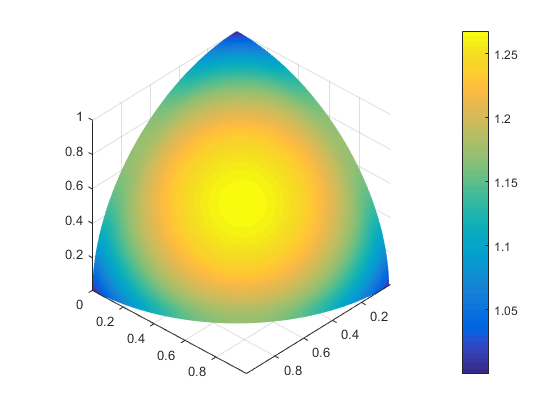
\includegraphics[width=0.75\textwidth]{cstar_blochsphere.png}
\caption{Heatmap showing the inverse stabilizer fidelity, $F(\psi)^{-1}$, for all single-qubit states lying in a single quadrant of the Bloch sphere. We note that the state with the largest inverse fidelity, and thus largest stabilizer extent, is the face-type magic state. Figure taken from~\cite{Bravyi2018}.}
\label{fig:fidelity_heatmap}
\end{figure}
% Note tension between the exact and approximate measures
% E.g small angle rotations
% Have a larger exact rank than magic states
It is interesting to note that there is a tension between trying to minimize the exact or the approximate stabilizer rank. For example, consider the two classes of single-qubit magic state. While the face state has a smaller stabilizer fidelity that the edge-type states ---  in fact it has the smallest possible stabilizer fidelity, c.f.\ Fig~\ref{fig:fidelity_heatmap} --- both states have equivalent exact stabilizer rank. Alternatively, single-qubit states exponentially close to a stabilizer state will have a small approximate stabilizer rank, but have a larger exact stabilizer rank. In fact, for any single qubit state with stabilizer fidelity $\geq\frac{1}{\sqrt{2}}$, its approximate stabilizer rank will have an asymptotic scaling smaller than $2^{0.5t}$, the upper bound obtained from computational searches in Section~\ref{sec:exact_results}.\par
% Generally we have been able to prove only upper bounds
% Mention some effort by sergey bravyi but only valid for states w/ clifford symmetries
% Most strategies focus on families of states with Clifford symmetries
Finally, we note that all the results shown here serve only as upper bounds on the stabilizer rank. While stabilizer fidelity is capable of lower bounding the stabilizer extent, this is itself also an upper bound on the approximate stabilizer rank. Currently, the only lower bounds that have been explicitly proven apply to the case of the $\ket{T}$ state. It was argued in~\cite{Bravyi2015} that $\chi\left(\ket{H^{\otimes n}}\right)=\Omega\left(\sqrt{n}\right)$, based on constructing states with finite stabilizer rank but which require a large number of $T$ gates to create. In~\cite{Bravyi2018}, it was also shown that the approximate stabilizer rank $\chi_{\epsilon}\left(\ket{H^{\otimes n}}\right)=\Omega\left(F(H)^{-n}\epsilon^{-2}\right)$, but only under the assumption that the decomposition is built from the states $\ket{0}$ and $\ket{+}$, as used in the random codes construction.\par
Part of this difficulty likely arises from the fact that, as a sparse optimization problem, even approximately computing the optimal stabilizer rank is $\NP$-hard~\cite{Natarajan1995}. Currently, the best explicit lower bound is a complexity theoretic argument. It was shown by Dalzell that for any classical simulation of a Clifford+$T$ circuit must have a runtime that scales asymptotically as $2^{\gamma t}$, where $\gamma > \frac{1}{128}$, otherwise the polynomial hierarchy would collapse to the third level~\cite{Dalzell2017}. This result acts as a lower-bound on the approximate stabilizer rank of the $\ket{T}$ magic states, and is significantly looser than the current best known decompositions with $\gamma\approx 0.23$. It is a open question if this complexity theoretic argument can be tightened.\par
In the case of approximate stabilizer rank, we might also ask if alternative strategies for building decompositions could be yield a smaller approximate stabilizer rank.\par
For example, inspired by the random codes method, we might consider using Schumacher compression to efficiently encode many copies of a resource state~\cite{Schumacher1995}. In~\cite{Bravyi2016}, the authors compared the Shannon entropy of the $\ket{H}$ state with the asymptotic $2^{0.23t}$ scaling obtained using random codes, showing that it outperforms Schumacher compression. Figure~\ref{fig:compression_comparison}, taken from~\cite{Bravyi2017}, shows a similar analysis comparing the Shannon entropy with the stabilizer extent for $\ket{\theta}$ states as a function of the angle $\theta$. We can see that in fact, at small angles, Schumacher compression can achieve a smaller decomposition than sparsification. However, over most of the parameter range, the difference between sparsification method performs significantly better.\par
Alternatively, we could consider techniques that construct an approximate stabilizer state decomposition by discarding only the terms which contribute least to the overall decomposition. Indeed, an interesting feature of both the random codes and sparsification methods is that the resulting decompositions are uniform mixtures of the sampled stabilizer states.\par
In the most general case, the simulation overhead achieved by discarding terms is related to the notion of $\epsilon$-sparsity, namely how many terms in the decomposition can be discarded while retaining an additive error $\epsilon$ in the output distribution~\cite{Pashayan2017}. The notion of $\epsilon$-sparsity is closely related to the smooth max entropy $H_{max}^{\epsilon}$, the logarithm of the number of terms with coefficients $\left|c_{i}\right|>\epsilon$. An ideal truncation method of this type would have approximate stabilizer rank $2^{H_{max}^{\epsilon}}$, but as previously stated computing optimal sparse decompositions of this type constitutes an $\NP$-hard problem.\par
In some tensor network methods for classical simulation, such as \texttt{Rollright} and \texttt{qFlex}, the output state of the computation before measurement is broken up into a decomposition of largely independent states, which contribute roughly equally to the norm~\cite{Markov2018,Villalonga2018}. Thus, they can achieve an approximate fidelity $f$ by dropping all but a fraction $f$ of the states~\cite{Markov2018}. In practice, this method does slightly worse than the target fidelity due to small overlaps $\sim10^{-6}$ between states~\cite{Villalonga2018}, but the reduction in the number of terms achieved is significant.\par
The overlap between general $n$-qubit stabilizer states, in contrast, varies significantly from $0$ to $2^{-s}\,:\,s\in\left[1,n\right]$. The sparsification method works around this, using the fact that sampling states according to $\frac{c_{j}}{\norm{\va{c}}_{1}}$, the expectation value 
\[\mathbb{E}\left[\ket{\omega}\right]=\frac{\ket{\psi}}{\norm{c}},\]
i.e.\ the sampled states have equal norm on average~\cite{Bravyi2018}. Additionally, grouping like terms, we can see that in the sampled state
\[\mathbb{E}\left[\ket{\tilde{\psi}}\right]=\mathbb{E}\left[\frac{\norm{c}}{\chi_{\epsilon}}\sum_{i=1}^{\chi_{\epsilon}}\ket{\omega_{i}}\right] = \mathbb{E}\left[\norm{c}
\sum_{j}\frac{\#\ket{w_{j}}}{\chi_{\epsilon}}\ket{w_{j}}\right]=\norm{c}\sum_{j}p_{j}\ket{w_{j}}.\]
On average, then, building uniform decompositions in this way does effectively weight each stabilizer state according to its contribution to the decomposition. It might however be interesting to test alternative sampling strategies, such as sampling without replacement or excluding terms with a coefficient below some small threshold value.
\begin{figure}[H]
\centering
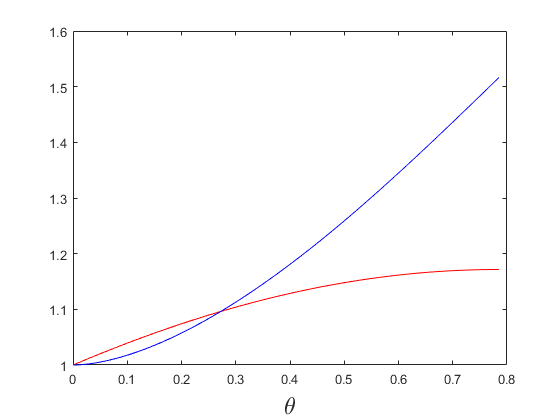
\includegraphics[width=0.75\textwidth]{Comparison.png}
\caption{Graph comparing the Shannon entropy (blue) and stabilizer extent (red) of $\ket{\theta}$ states, defined in Eq.~\ref{eq:theta_state}, as a function of the angle $\ket{\theta}$.}
\label{fig:compression_comparison}
\end{figure}